\begin{frame}{Solução Proposta: Processo de Desenvolvimento}
\begin{itemize}
	\item Processo de Desenvolvimento Adotado: \alert{Processo Unificado Ágil}
	\ \ \newline
	\item Aplicação a ser desenvolvida não é considerada de grande porte
	\ \ \newline
	\item Papéis:
	\begin{itemize}
		\item Desenvolvedor e testador: Pedro Augusto
		\item Cliente: Profa. Maria Betânia
		\item Solicitante do software e Gerente do Projeto: Profa. Elloá
	\end{itemize}
\end{itemize}
\end{frame}

\begin{frame}{Solução Proposta: Diagramas de Caso de Uso}
\begin{figure}[h!]
\centering
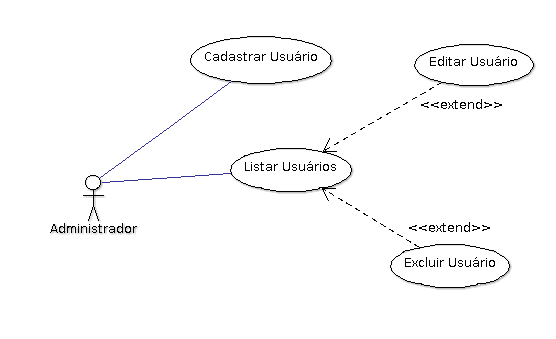
\includegraphics[width=0.8\linewidth]{./img/uc001}
%\caption{Módulo Gerencia Conta de Usuário} \label{fig:uc001}
\end{figure}
\end{frame}

\begin{frame}{Solução Proposta: Diagramas de Caso de Uso}
\begin{figure}[h!]
\centering
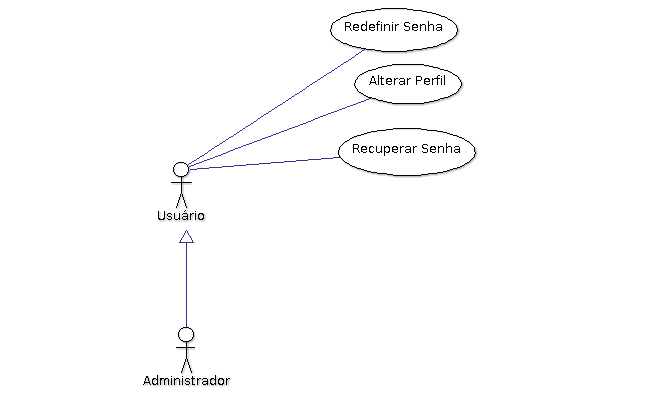
\includegraphics[width=0.7\linewidth]{./img/uc002}%
%\caption{Módulo Usuário} \label{fig:uc001}
\end{figure}
\end{frame}

\begin{frame}{Solução Proposta: Diagramas de Caso de Uso}
\begin{figure}[h!]
\centering
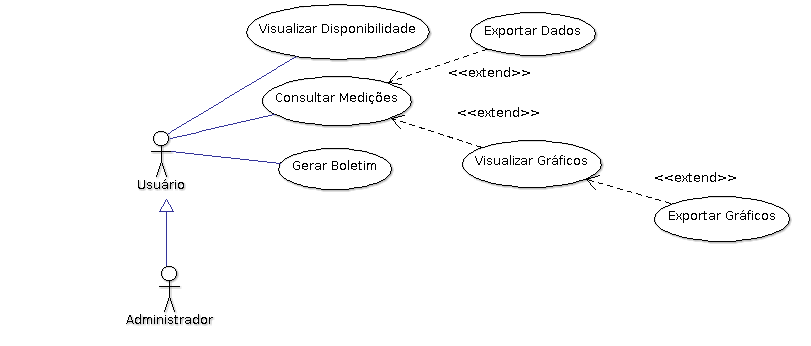
\includegraphics[width=1\linewidth]{./img/uc003}
%\caption{Módulo Consulta Medições} \label{fig:uc001}
\end{figure}
\end{frame}

\begin{frame}{Solução Proposta: Diagramas de Caso de Uso}
\begin{figure}[h!]
\centering
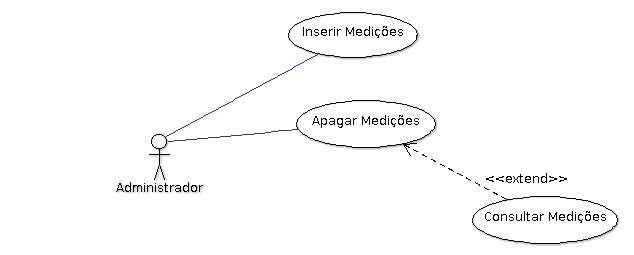
\includegraphics[width=1\linewidth]{./img/uc004}
%\caption{Módulo Gerencia Medições} \label{fig:uc001}
\end{figure}
\end{frame}

\begin{frame}{Solução Proposta: Prototipação}
\begin{figure}[h!]
\centering
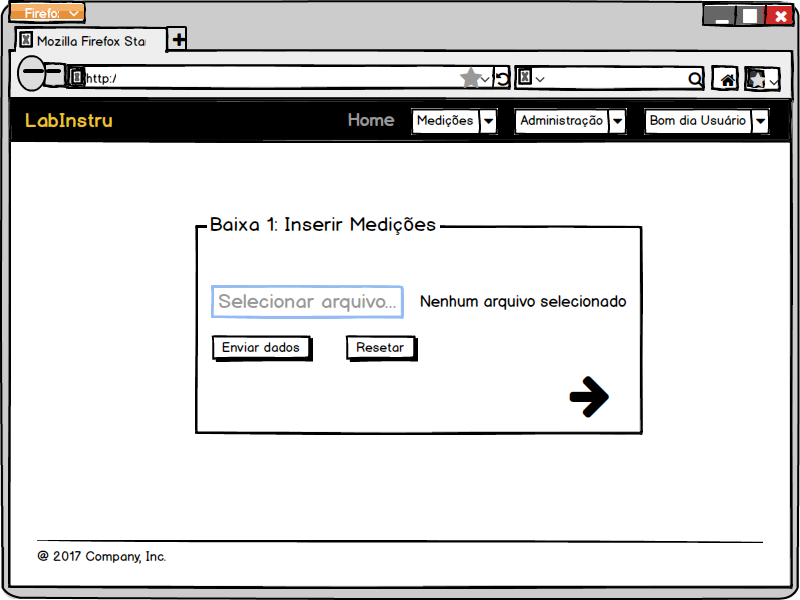
\includegraphics[width=0.6\linewidth]{./img/tela053}
\caption{Protótipo cadastra medições} \label{fig:uc001}
\end{figure}
\end{frame}

\begin{frame}{Solução Proposta: Prototipação}
\begin{figure}[h!]
\centering
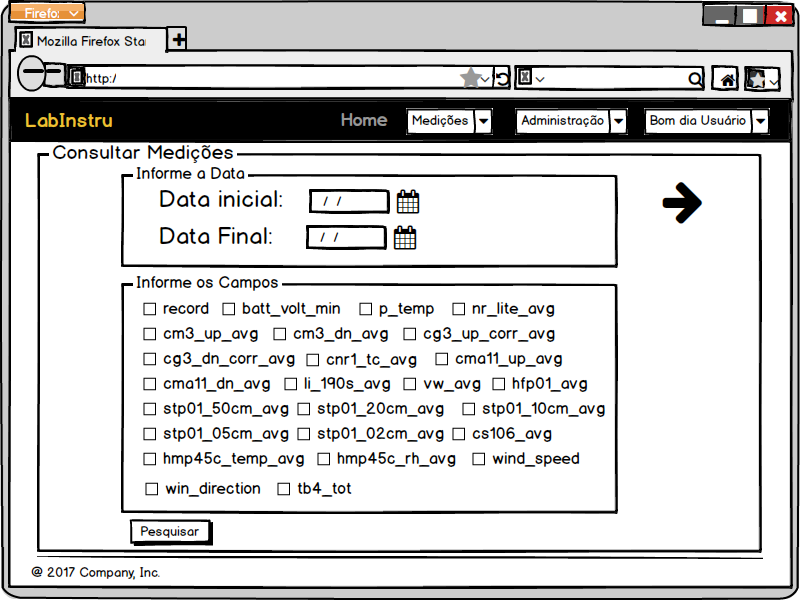
\includegraphics[width=0.6\linewidth]{./img/tela058}
\caption{Protótipo consulta medições} \label{fig:uc001}
\end{figure}
\end{frame}

\begin{frame}{Solução Proposta: LabInstru Web}
\begin{itemize}
	\item \alert{LabInstru Web}: plataforma web proposta para atender às necessidades identificadas no LabInstru
	\ \ \newline
	\item \emph{Framework} utilizado: Web2py
		\begin{itemize}
			\item Programável e escrito em Python
			\item Utiliza o MVC como padrão de projeto
		\end{itemize}
	\ \ \newline
	\item Melhorias na interface com o usuário:
	\begin{itemize}
		\item \emph{Framework} Bootstrap
		\item Biblioteca JQuery
	\end{itemize}
	\ \ \newline
	\item Sistema gerenciador de Banco de Dados: MySQL
\end{itemize}
\end{frame}

\begin{frame}{Solução Proposta: Funcionalidades Implementadas}
\begin{figure}[h!]
\centering
\frame{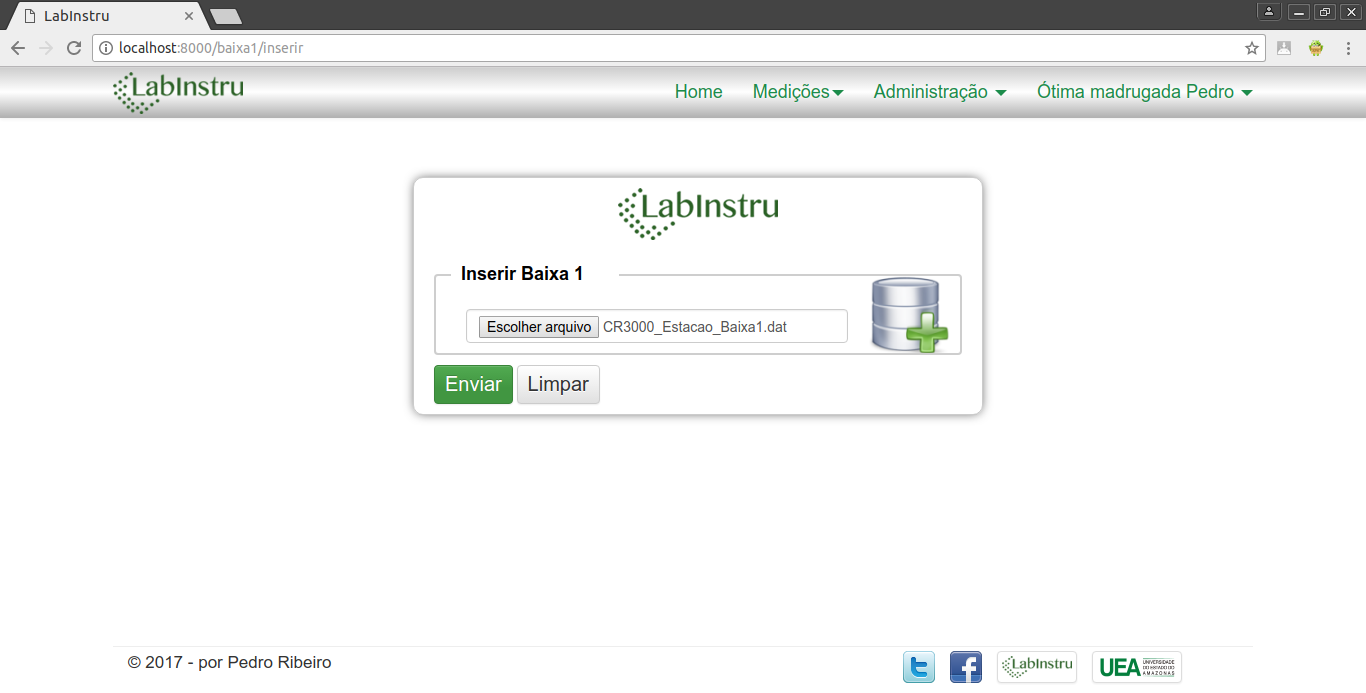
\includegraphics[width=0.7\linewidth]{./img/ap12}}
\caption{Cadastro de Medições.} \label{fig:uc001}
\end{figure}
\end{frame}

\begin{frame}{Solução Proposta: Funcionalidades Implementadas}
\begin{figure}[h!]
\centering
\frame{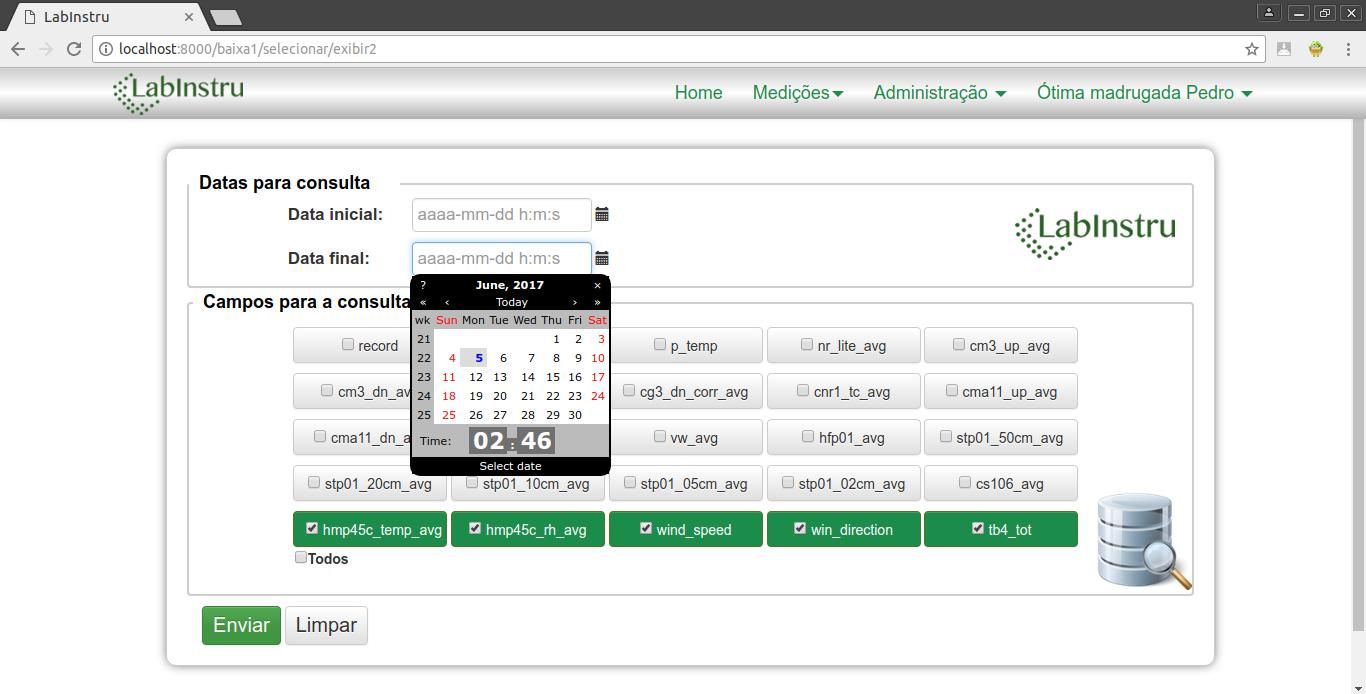
\includegraphics[width=0.7\linewidth]{./img/ap3}}
\caption{Consulta de medições.} \label{fig:uc001}
\end{figure}
\end{frame}

\begin{frame}{Solução Proposta: Funcionalidades Implementadas}
\begin{figure}[h!]
\centering
\frame{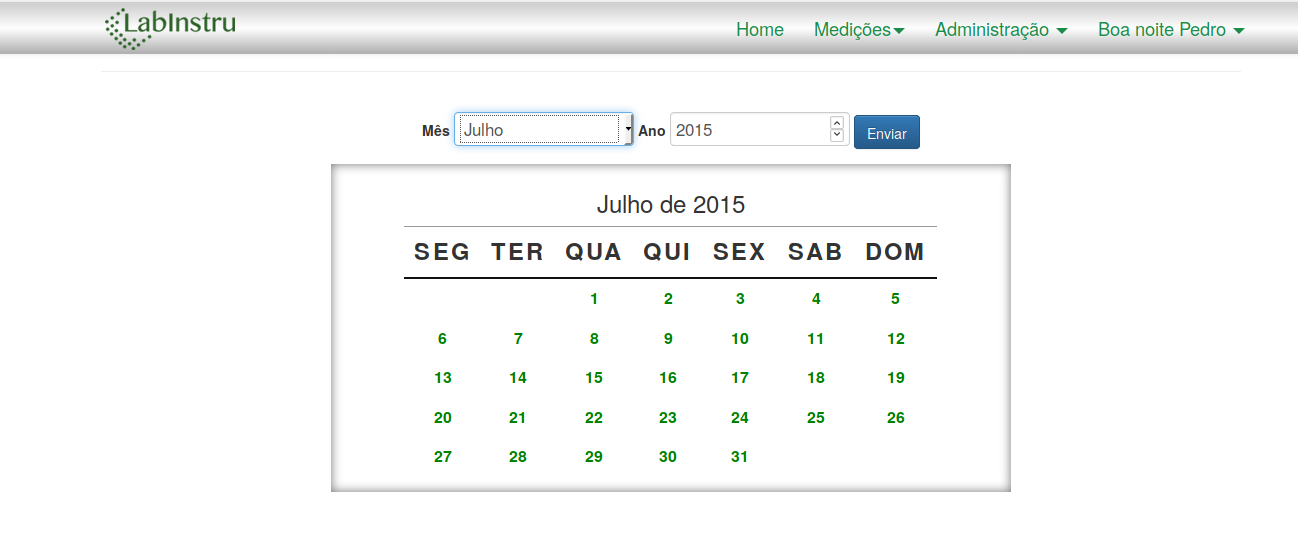
\includegraphics[width=0.7\linewidth]{./img/disponibilidade2}}
\caption{Verificação de disponibilidade} \label{fig:disponibilidade}
\end{figure}
\end{frame}

\begin{frame}{Apresentação LabInstru Web}
	\begin{center}
	\movie[width=160px, height=90px, externalviewer]{Vídeo de ilustração de algumas funcionalidades.}{video/video.mp4}
	\end{center}
\end{frame}

\begin{frame}{Modelo para Boletim Meteorológico Diário}
\begin{itemize}
	\item Uma das atividades promovidas pelo LabInstru
	\item Importante informativo sobre clima e tempo de nossa região
\item Divulgação das informações junto à comunidade
	\ \ \newline
	\item Possui várias informações derivadas dos dados obtidos da estação meteorológica
	\begin{itemize}
		\item Índice de Calor
		\item Escala de Beaufort
	\end{itemize}
	\ \ \newline

	\item Elaboração de modelo para o boletim meteorlógico
\end{itemize}
\end{frame}

\begin{frame}{Modelo para Boletim Meteorológico Diário}
\begin{figure}[h!]
\centering
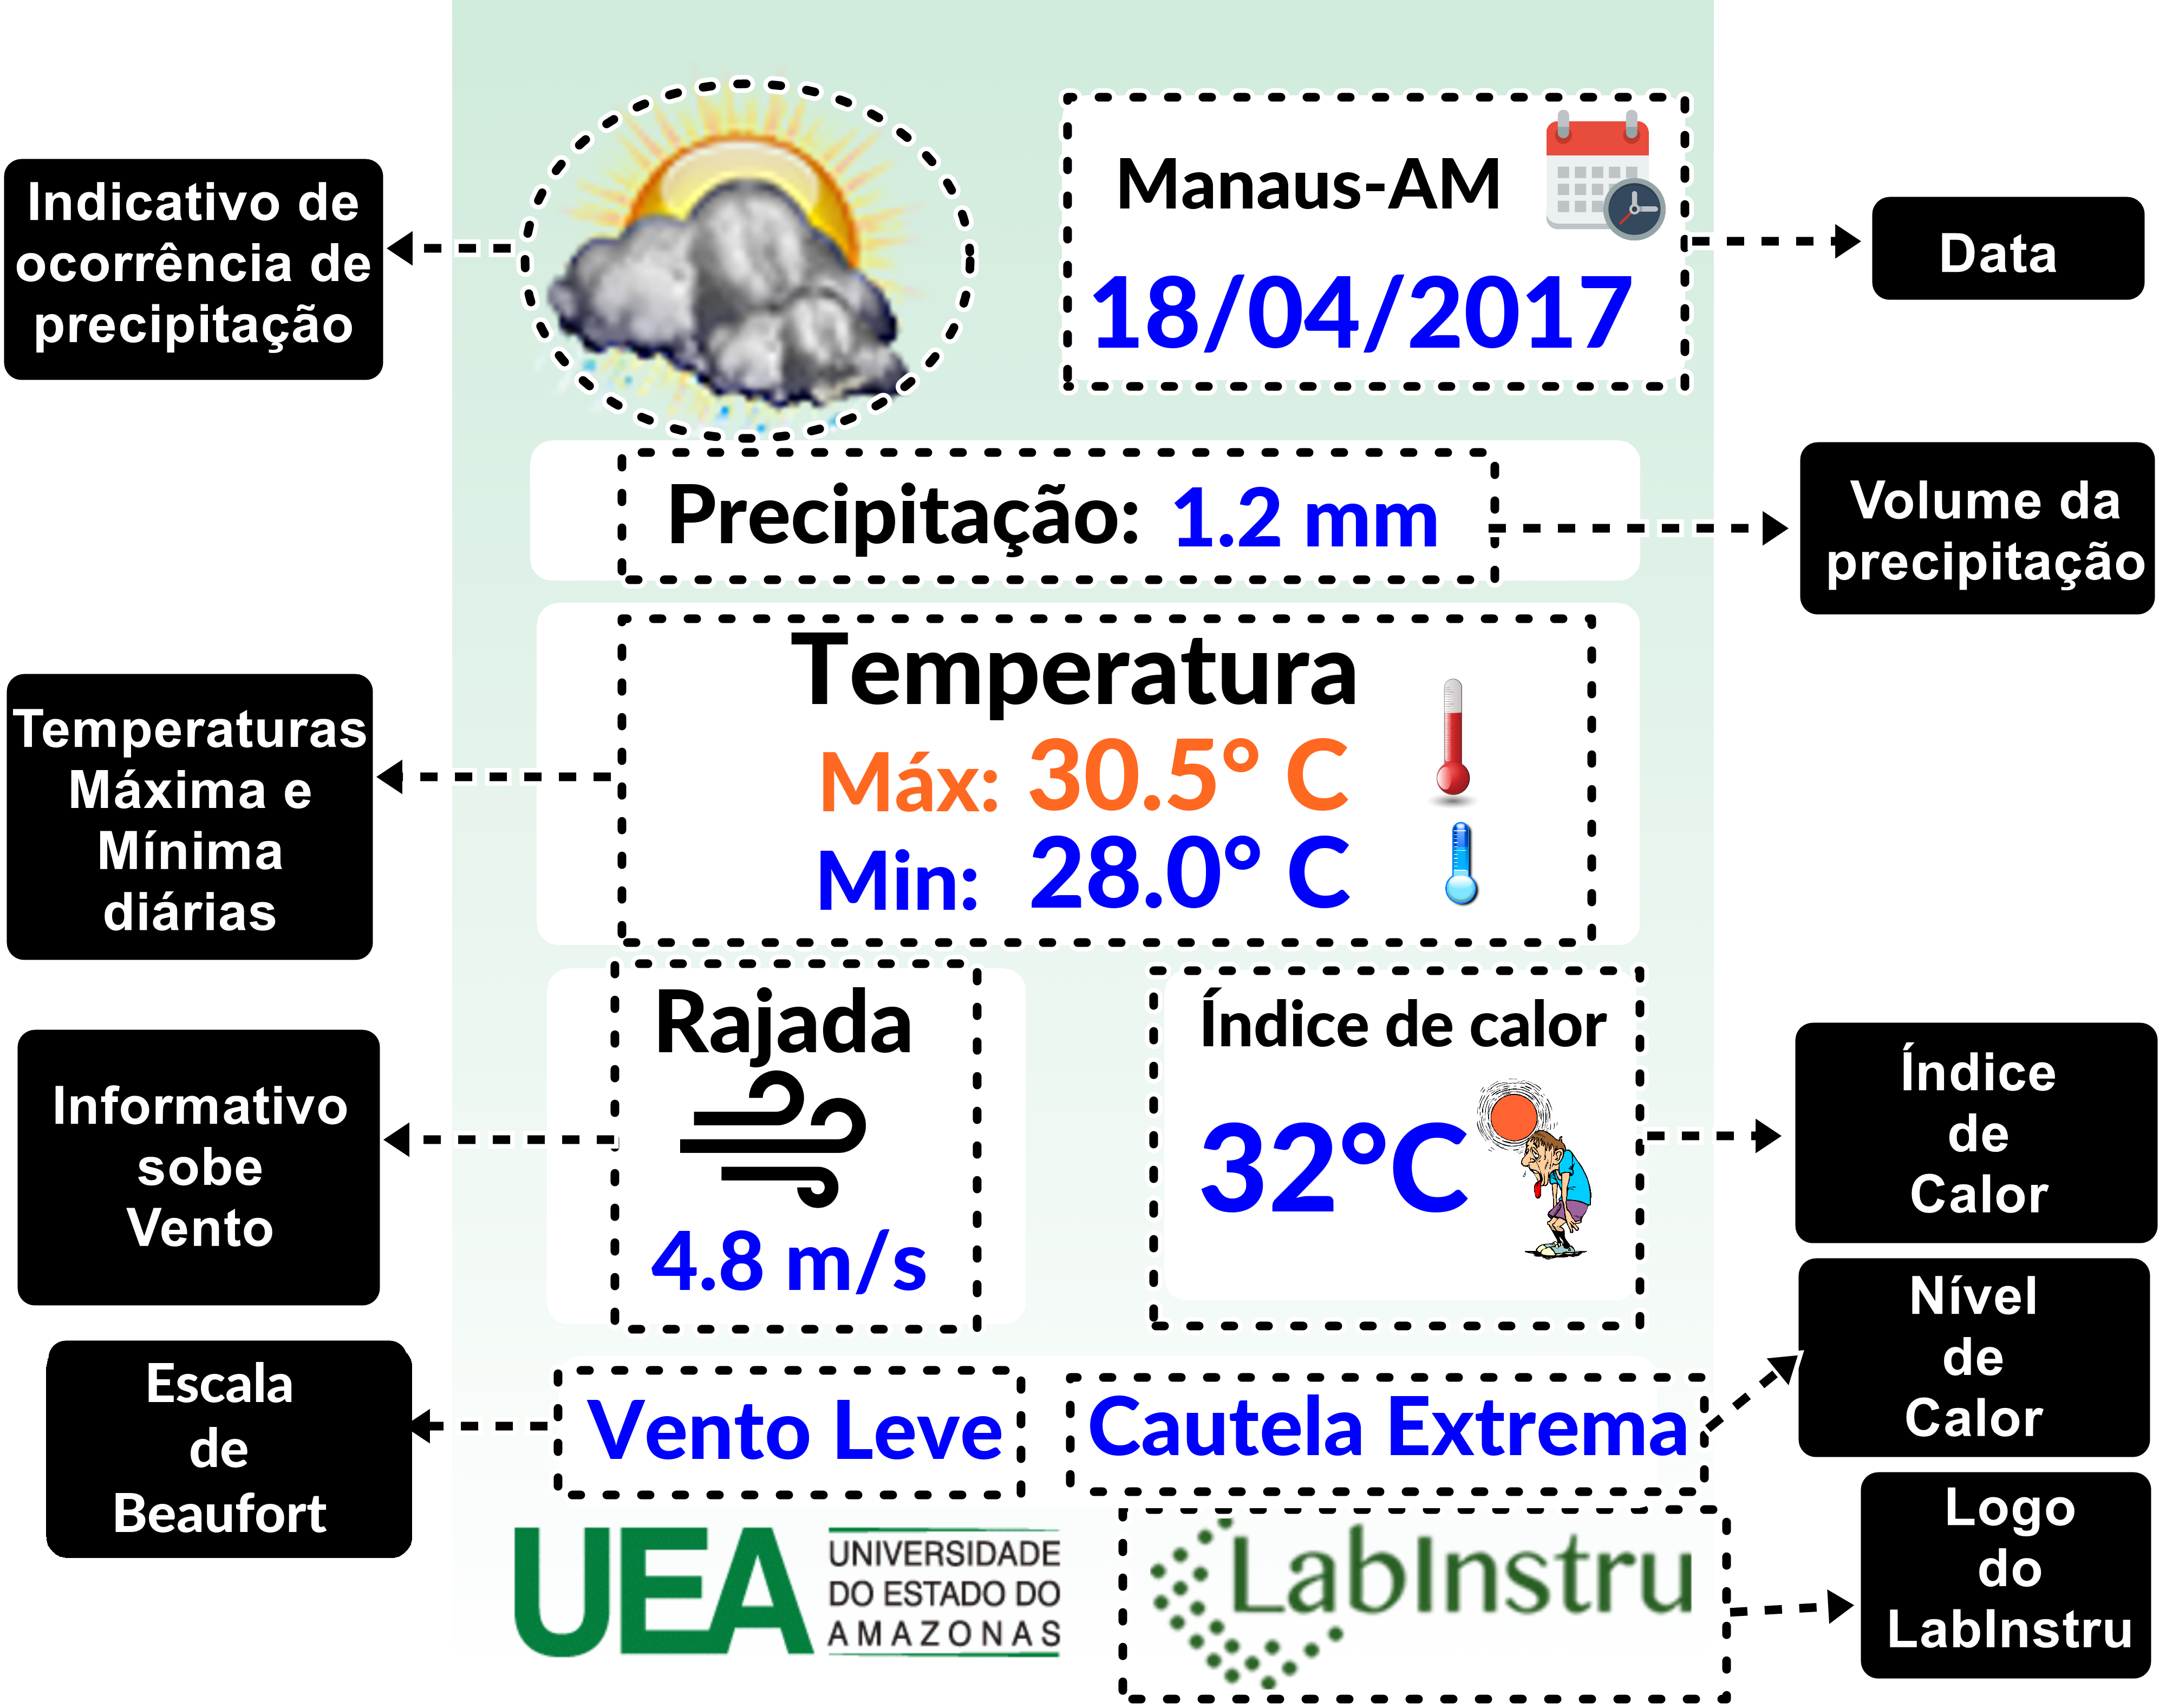
\includegraphics[width=0.5\linewidth]{./img/esbocoBoletim}
\caption{padrão a seguir o Boletim Meteorológico} \label{fig:modeloBoletim}
\end{figure}
\end{frame}

\begin{frame}{Boletim Meteorológico Diário}
\begin{figure}[h!]
\centering
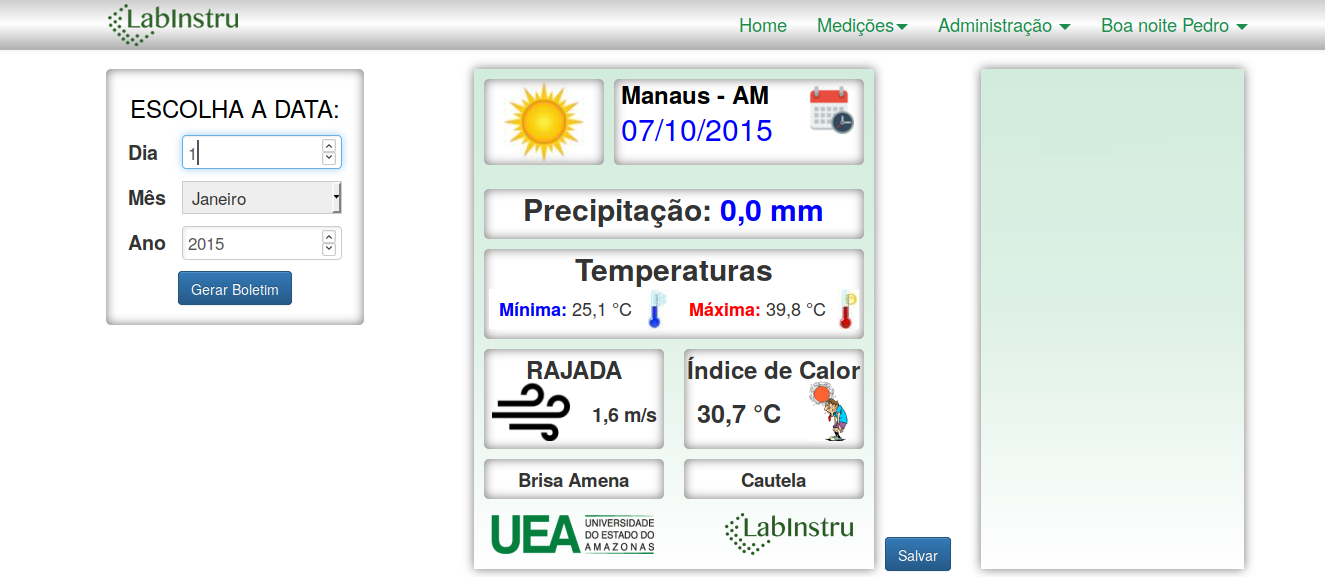
\includegraphics[width=0.7\linewidth]{./img/boletim}
\caption{Boletim Meteorológico Implementado} \label{fig:boletim}
\end{figure}
\end{frame}

\begin{frame}{Métricas de Software}
\begin{itemize}
\item Linhas de código: 7264 no total
\begin{itemize}
\item[-] Arquivos Python:1714 linhas
\ \ \newline
\item[-] Arquivos HTML:2400 linhas
\ \ \newline
\item[-] Arquivos de estilo: 3150 linhas
\end{itemize}
\item Funções disponíveis no Controller: 28
\ \ \newline
\item Modelo de dados: 8
\end{itemize}
\end{frame}
